\begin{figure*}[!t]
        \centering{
                \begin{tabular}{cccc}
                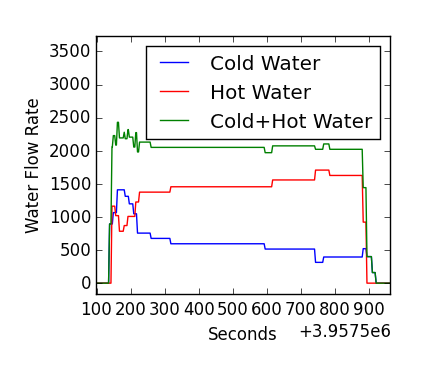
\includegraphics[width=1.6in]{multidisaggfig/shower.png}&
                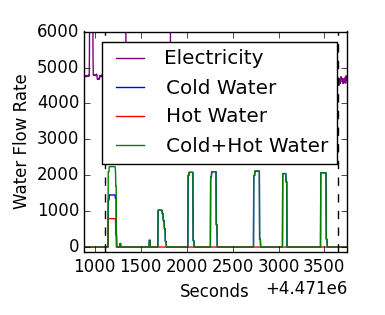
\includegraphics[width=1.6in]{multidisaggfig/washingMachineWater.png}&
                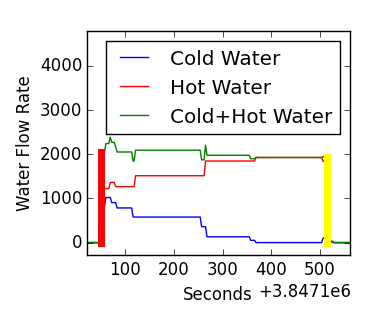
\includegraphics[width=1.6in]{multidisaggfig/showerFitted.png}&
                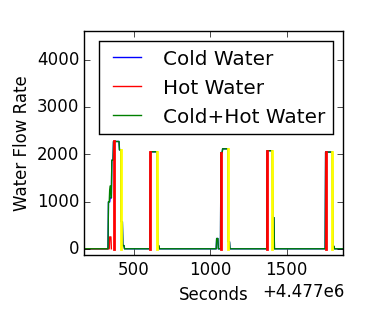
\includegraphics[width=1.6in]{multidisaggfig/washingMachineWaterFitted.png}
                \tabularnewline
                (a) & (b) & (c) & (d) \tabularnewline
                \end{tabular}
                }
        \caption{
        (a) and (b) describe complete usage cycle of shower and washing machine in dataset study10. X-axis is the duration to a specific time in seconds, Y-axis is water flow rate in 10000*liter/minute. 
The dash line denotes the on and off event of washing machine electricity usage. (c) and (d) denote the water disaggregation of shower and washing machine. The fitted red line denotes the on of water, and the fitted yellow line denotes the off of water. }
        \label{fig_showerWashingMachine}
\end{figure*}